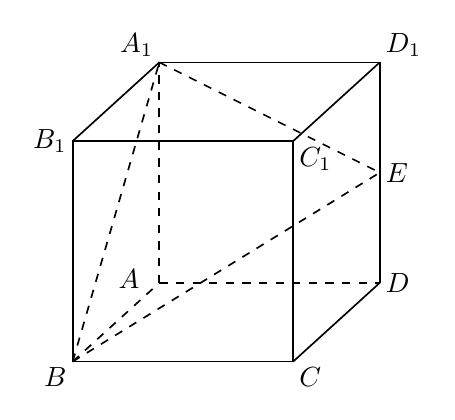
\begin{tikzpicture}[x=1cm,y=1cm,font=\normalsize,
  geometry edge/.style={solid,line width=.6pt},
  geometry label/.style={font=\normalsize,inner sep=2pt}]
\coordinate (B) at (0,0);
\coordinate (C) at (2.8,0);
\coordinate (B1) at (0,2.8);
\coordinate (C1) at (2.8,2.8);
\coordinate (A) at (1.1,1.0);
\coordinate (D) at (3.9,1.0);
\coordinate (A1) at (1.1,3.8);
\coordinate (D1) at (3.9,3.8);
\coordinate (E) at (3.9,2.4);
\draw[geometry edge] (B)--(C);
\draw[geometry edge] (C)--(D);
\draw[geometry edge] (B)--(B1)--(C1)--(C);
\draw[geometry edge] (A1)--(D1)--(D);
\draw[geometry edge] (A1)--(B1);
\draw[geometry edge] (C1)--(D1);
\draw[geometry edge,dashed] (B)--(A);
\draw[geometry edge,dashed] (A)--(D);
\draw[geometry edge,dashed] (A)--(A1);
\draw[geometry edge,dashed] (B)--(A1);
\draw[geometry edge,dashed] (B)--(E);
\draw[geometry edge,dashed] (A1)--(E);
\node[geometry label,below left] at (B) {$B$};
\node[geometry label,below right] at (C) {$C$};
\node[geometry label,right] at (D) {$D$};
\node[geometry label,below left,xshift=-5pt,yshift=7pt] at (A) {$A$};
\node[geometry label,left] at (B1) {$B_{1}$};
\node[geometry label,below right] at (C1) {$C_{1}$};
\node[geometry label,above left] at (A1) {$A_{1}$};
\node[geometry label,above right] at (D1) {$D_{1}$};
\node[geometry label,right] at (E) {$E$};
\end{tikzpicture}
